\documentclass[12pt]{article}
\usepackage[utf8]{inputenc}
\usepackage{multicol}
\usepackage{amsmath}
\usepackage{setspace}
\usepackage{graphicx}
\usepackage{caption}
\usepackage{float}
\usepackage{geometry}
\usepackage{subcaption}
\geometry{margin=1in}
\usepackage{graphbox}
\graphicspath{ {figures/} }


\title{Robust testing using Tukey's one df interaction model}
\author{Wenxing (Blue) Wang }
%\date{June 2021}


\begin{document}
\maketitle

\noindent Keywords: Bootstrap, Hypothesis testing, Robust regression, Tukey 1 df regression.

\section{Introduction}

Researches of last recent decades in biomedical areas have been largely promoted by genome-wide association studies (GWASs) (Hindorff et al., 2009). Studies focusing on exploration of contribution of genes to disease have driven the targeted-oriented development medicine. Among these researches, SNPs has been an important focus. For example, a study in 2013 has explored the association between 67 SNPs and breast cancer (Michailidou et al., 2013). Therefore, statistical models have been proposed in past years to evaluate the contributions of SNPs to disease and to explain some of the properties of targeted genes such as heritability.

One of the major problems of study of SNPs is the association of genes in their contributions to disease. There could be direct interactions between genes (Jia et al., 2000) and there could also be interactions between proteins coded by genes (Titeca, Lemmens, Tavernier \& Eyckerman, 2019). SNPs can also be used as markers in linkage disequilibrium (LD) with potential causal variants (Gibbs et al., 2003). These types of association could be complex and evaluation of gene contributions to phenotypes under such association is also a hard problem. Chatterjee (2006) and his collaborators proposed a parsimonious model that incorporates gene-gene and gene-environment interactions with a Tukey’s 1-df model of interaction (Tukey, 1949). It is a logistic regression model that incorporates two groups of covariates that represents two genes with several SNPs and one term of interaction of these two genes. The response is a binary clinical measurement of the individual. They also designed a test statistic to evaluate the contribution of a single gene to the disease under the association between this gene and another gene or environment based on the model. This model, according to researchers in the past decade, have efficiently exploited LD pattern of SNPs in a gene and associations of gene-gene and gene-environment (Wang, Li \& Wei, 2015) (Mukherjee, Ahn, Gruber \& Chatterjee, 2012).

However, measurements as responses in this model are binary since the model is based on logistic regression. Therefore, this kind of model can only be applied on cases with binary clinical measurements. Chatterjee (2006) used the example whether the patient was diagnosed with cancer as the response to conduct the simulation studies. Novel methods are needed for cases involving continuous measurements as responses such as the concentration of plasma glucose of diabetes patients, the blood pressure of patients with cardiovascular disease. These data can also be important in biomedical experiments and drug developments.

In this article, we proposed a model mainly based on the model developed by Chatterjee (2006) and his collaborators. While keeping the part of Tukey’s 1-df model of interaction, in contrast to taking logistic regression as the major part of the model, this model is based on linear regression with continuous values as the response. Furthermore, we discussed methods to deal with possible outliers in clinical data. We proposed the absolute loss function for the calculation of test statistics. Apart from the regression methods and loss functions applied, derivation of the test statistics is based on the method by Chatterjee (2006) and his team. We simulated case-control data to evaluate type I errors and powers of the test statistic based on linear regression with absolute loss function. We also conducted simulation studies to test the ability of outlier resistance of the test statistic derived with absolute loss function by comparing the type I errors and powers of test statistics derived with absolute loss function and squared loss function. We also applied this model to datasets with genomic data and clinical data collected from a group of diabetes patients (Jablonski et al., 2010). All simulation study results demonstrate major power advantages for the proposed methods in terms of study of gene-gene and gene-environment association with continuous responses. Properties such as robustness (resistance to outliers) of test statistic derived with absolute loss function over the test statistic derived with squared loss have also been demonstrated.

\section{Method}

\subsection{Test statistics}
The Tukey's 1-df interaction model takes the formula:
\begin{displaymath}
Y_i = \alpha + S_{i1}^T\beta_1 + S_{i2}^T\beta_2 + \gamma (S_{i1}^T\beta_1) (S_{i2}^T\beta_2) + e_i
\end{displaymath}
with the null hypothesis
$$
H_0: \beta_1 = 0
$$
Following the protocol proposed in previous work (Chatterjee et al., 2006), the steps for deriving the test statistics are
\begin{enumerate}
    \item Obtain the maximum-likelihood estimates for $\alpha, \beta_2$ and $\sigma$ under null hypothesis $H_0$. The model becomes a standard linear regression with the estimates $\hat{\psi} = (\hat{\alpha}, \hat{\sigma}, \hat{\beta_2})$
    \item For a fixed value $\theta$, evaluate the score functions for the parameters $\beta_1$ at $\beta_1 = 0$, $\psi = \hat{\psi}$ and $\theta = \gamma$, that is
    $$
    S_{\beta_1}(\theta) = \frac{dl}{d\beta_1}\mid_{\beta_1 = 0, \psi = \hat{\psi}, \gamma = \theta}
    $$
    \item Estimate the inverse of the variance-covariance matrix for $S_{\beta_1}(\theta)$ with
    $$
    I^{\beta_1 \beta_1}(\theta)=\left[I_{\beta_1 \beta_1}(\theta)-I_{\beta_1 \psi}(\theta) I_{\psi \psi}^{-1} I_{\psi \beta_1}(\theta)\right]^{-1}
    $$ 
    where the expressions for the component information matrices $I_{\beta_1 \beta_1}(\theta)=\partial l / \partial \beta_1 \partial \beta_1^T, I_{\beta_1 \psi}(\theta)=\partial l / \partial \beta_1 \partial \psi^T$ and $I_{\psi \psi}=\partial l / \partial \psi \partial \psi^T$, evaluated at $\beta_1=0$ and $\psi=\hat{\psi}$ are given in the formula
    \item For fixed value of $\theta$, obtain the score statistics
    $$
    T_1(\theta)=S_{\beta_1}(\theta)^T I^{\beta_1 \beta_1}(\theta) S_{\beta_1}(\theta).
    $$
    Compute the final test statistics as $T_1^*=\max _{L \leq \theta \leq U} T(\theta)$, where $L$ and $U$ denote some prespecified values for lower and upper limits of $\theta$, respectively.
\end{enumerate}
\subsubsection{Gaussian residual}
Under Gaussian assumptions on the residual when $e_i$ are i.i.d $N(0, \sigma^2)$ errors, the log likelihood function is denoted as
$$
l = -\frac{n}{2}\log(2\pi\sigma^2) -  \sum_{i=1}^n [Y_i - \alpha - S_{i1}^T\beta_1 - S_{i2}^T\beta_2 - \gamma (S_{i1}^T\beta_1) (S_{i2}^T\beta_2)]^2/(2\sigma^2)
$$
The score function for $\beta_1$ is
$$
S_{\beta_1}(\theta) = \frac{\partial l}{\partial \beta_1} =   \sum_{i=1}^n S_{i1}\{1 + \gamma S_{i2}^T\beta_2 \}e_i/\sigma^2
$$
when
$$
e_i = Y_i - \alpha - S_{i1}^T\beta_1 - S_{i2}^T\beta_2 - \theta (S_{i1}^T\beta_1) (S_{i2}^T\beta_2)
$$
for the given
$$
\gamma = \theta
$$
The variance-covariance matrix of the estimated score function is
$$
I = \begin{bmatrix}
I_{\beta_{1}\beta_{1}} &  I_{\beta_{1}\alpha}  & I_{\beta_{1}\beta_{2}} & I_{\beta_{1}\sigma^2}\\
I_{\beta_{1}\alpha} & I_{\alpha\alpha} & I_{\alpha\beta_{2}} & I_{\alpha\sigma^2} \\
I_{\beta_{2}\beta_{1}} & I_{\beta_{2}\alpha} & I_{\beta_{2}\beta_{2}} & I_{\beta_{2}\sigma^2}\\
I_{\sigma^2\beta_{1}} & I_{\sigma^2\alpha} & I_{\sigma^2\beta_{2}} & I_{\sigma^2\sigma^2}
\end{bmatrix}
$$
Each part of the matrix are
\begin{equation*}
    I_{\alpha\beta_1} = E[\sum_{i=1}^n S_{i1}\{1 + \theta S_{i2}^T\beta_2 \}e_i^2/\sigma^4] = \sum_{i=1}^n S_{i1}\{1 + \theta S_{i2}^T\beta_2 \}/\sigma^2
\end{equation*}

\begin{equation*}
   I_{\alpha\beta_2} = E[\sum_{i=1}^n S_{i2}\{1 + \theta S_{i1}^T\beta_1 \}e_i^2/\sigma^4] = \sum_{i=1}^n S_{i2}\{1 + \theta S_{i1}^T\beta_1 \}/\sigma^2
\end{equation*}

\begin{equation*}
   I_{\beta_1\beta_1} = E[\sum_{i=1}^n S_{i1}S_{i1}^T\{1 + \theta S_{i2}^T\beta_2 \}^2e_i^2/\sigma^4] = \sum_{i=1}^n S_{i1}S_{i1}^T\{1 + \theta S_{i2}^T\beta_2 \}^2/\sigma^2
\end{equation*}

\begin{equation*}
    \begin{aligned}
I_{\beta_1\beta_2} &= E[\sum_{i=1}^n S_{i1}S_{i2}^T\{1 + \theta S_{i1}^T\beta_1 \}\{1 + \theta S_{i2}^T\beta_2 \}e_i^2/\sigma^4]\\ &=\sum_{i=1}^n S_{i1}S_{i2}^T\{1 + \theta S_{i1}^T\beta_1 \}\{1 + \theta S_{i2}^T\beta_2 \}/\sigma^2
    \end{aligned}
\end{equation*}

\begin{equation*}
   I_{\beta_2\beta_2} = E[\sum_{i=1}^n S_{i2}S_{i2}^T\{1 + \gamma S_{i1}^T\beta_1 \}^2e_i^2/\sigma^4] = \sum_{i=1}^n S_{i2}S_{i2}^T\{1 + \theta S_{i1}^T\beta_1 \}^2/\sigma^2
\end{equation*}

\begin{equation*}
I_{\beta_0\sigma^2} = 0,\;
I_{\beta_1\sigma^2} = 0, \;
I_{\beta_2\sigma^2} = 0
\end{equation*}
\begin{equation*}
I_{\sigma^2\sigma^2}  = E[\{-\frac{n}{2\sigma^2} + \sum_{i=1}^n e_i^2/(2\sigma^4)\}^2] = \text{var}[\sum_{i=1}^n e_i^2/(2\sigma^4)] = \frac{n}{2\sigma^4}
\end{equation*}
and also
\begin{equation*}
I_{\beta_1\psi}=
\left[\begin{matrix}
I_{\beta_{1}\alpha}  & I_{\beta_{1}\beta_{2}} & I_{\beta_{1}\sigma^2}
\end{matrix}
\right]
\end{equation*}
\begin{displaymath}
I_{\psi\psi}=
\begin{bmatrix}
I_{\alpha\alpha} & I_{\alpha\beta_{2}} & I_{\alpha\sigma^2} \\
I_{\beta_{2}\alpha} & I_{\beta_{2}\beta_{2}} & I_{\beta_{2}\sigma^2}\\
I_{\sigma^2\alpha} & I_{\sigma^2\beta_{2}} & I_{\sigma^2\sigma^2}
\end{bmatrix}
\end{displaymath}
\subsubsection{Laplace residual}
We have also tried the Laplace assumption on $e_i$, expecting more robust performance when dealing with datasets containing outliers. Under this assumption $e_i$ follows Laplace distributions with scale $b = \sigma$
Denote 
$$
\mu_i=\alpha + S_{i1}^T\beta_1 + S_{i2}^T\beta_2 + \gamma (S_{i1}^T\beta_1) (S_{i2}^T\beta_2)
$$
the log likelihood function is
\begin{displaymath}
l=-\log \sigma -\dfrac {\sum ^{n}_{i=1}\left| Y_{i}-\mu _{i}\right| }{2\sigma ^{2}}
\end{displaymath}
and the score function is
\begin{displaymath}
S_{\beta_1}(\theta) = \dfrac {-\sum ^{n}_{i=1}\text{sign}\left( Y_{i}-\mu_{i} \right) S_{1i}\left( 1+\theta S_{2i}\beta _{2i}\right) }{2\sigma ^{2}}
\end{displaymath}
To resolve the issue that the derivative of the score function will be 0 due to the sign function, we consider the asymptotic test with large samples. When sample size is sufficiently large, the conclusion holds that
$$
S_{\beta_1}(\theta)\mid_{\hat{\psi}}\rightarrow S_{\beta_1}(\theta)\mid_{\psi}
$$
when $\hat{\psi}$ is the maximum likelihood estimation of $\psi$. Then
\begin{displaymath}
\text{Var}\left[ S\left( \beta _{{1p}}\right) \right] =\dfrac {\sum ^{n}_{i=1}S^{2}_{1pi}\left( 1+\gamma S_{2i}\beta _{2i}\right)^2 }{4\sigma ^{4}}
\end{displaymath}
for the $p^{th}$ value in vector $\beta_1$ and also
\begin{displaymath}
\text{Cov}[ S( \beta _{{1p}}),S( \beta_{1q})]=
\dfrac {\sum ^{N}_{i=1}S_{1pi} S_{1qi}\left( 1+\gamma S_{2i}\beta _{2i}\right)^2 }{4\sigma ^{4}}
\end{displaymath}
for the $p^{th}$ value and $q^{th}$ in vector $\beta_1$ and also and $p\neq q$.


\subsection{Permutation test}
When hard to derive the null distribution of the test statistic in both finite sample case and large sample case, we consider the permutation test to finish the hypothesis testing. We adopted the method is proposed by Freedman and Lane (1983) with the steps:
\begin{enumerate}
    \item Estimate the value of $\beta_2$ under the null hypothesis that $\beta_1=0$

\item  Plug in the estimator in the reduced model and get the residual for each sample 

\item Permute the residues randomly and produce $R_{Y \mid X}^{*}$ 

\item  New values of $Y^{*}$ are calculated by adding $R_{Y \mid X}^{*}$ to the fitted  values, that is $Y^{*}=\hat\alpha+S_2\hat{\beta_{2}}+R_{Y \mid X}^{*}$ 

\item  Compute the test statistic with $Y^{*}$ obtained before and covariates.

\end{enumerate}

\section{Simulation Study}

We evaluated the performance of the proposed hypothesis testing with simulation studies. We compared Type I error rates and powers of the proposed hypothesis testing and several different statistical methods. In the simulated datasets, the response is generated by
$$
Y_i = \alpha + S_{i1}^T\beta_1 + S_{i2}^T\beta_2 + \gamma (S_{i1}^T\beta_1) (S_{i2}^T\beta_2)+\epsilon_i
$$
where $S_{1}$ and $S_{2}$ are two groups of covariates generated from a standard Gaussian distribution and $\beta_1$ and $\beta_2$ are two vectors with the length of 5. All values within the same vector of $\beta_1$ or $\beta_2$ are set to be identical, where $\beta_2 = 0.2*1_5$ and $1_k$ represents a vector of length $k$ with each element being $1$. We set $\beta_1 = \delta * 1_5$ for some constant $\delta$. We set $\delta = 0$ to evaluate type I error, and vary $\delta$ from  $0.1$ to $0.8$ to evaluate power of our test. We have also set $\alpha=3$ and $\gamma=1$

To assess the robustness of the proposed test, the value of $\epsilon$ is generated with 4 different distributions prone to produce outliers, which are Laplace distribution, logistic distribution, Cauchy distribution and mixed distribution that contains two Gaussian distributions with different variances. The details of $\epsilon$ generation are in table 1.

We use B = 200 bootstrap samples for each simulated dataset. We first compute the observed test statistic, and then compute B bootstrapped test statistics under null hypothesis. We compute the p-value as the proportion of the bootstrapped test statistics larger than the observed test statistic. Specifically
$$
p = \sum I(T_b > T_{obs})/B
$$
The process was repeated 1000 times with one specific group of parameters and for each time, the p-value was recorded. There are in total 4 groups of parameters with each one containing a sample size of 50, 100, 200 and 500. Finally among these 1000 values, the percentage that the value is smaller than or equal to a given level of significance, for example, 0.05 was recorded.

To evaluate power, we used the same method of bootstrap samples for each simulated dataset. The process was repeated 300 times with one specific group of parameters and for each time, the p-value was recorded. Apart from different values for $\beta_1$ 4 different sample sizes of 50, 100, 200 and 500 were also applied in each different group of parameters. Finally, among these 300 values, the percentage of values smaller than or equal to 0.05 were recorded.

\begin{table}
\centering
\begin{tabular}{llllll}
\hline
 & &  
\multicolumn{2}{l}{$n = 50$} & \multicolumn{2}{l}{$n = 100$} \\
\hline
Configuration & Distribution & Absolute & Square & Absolute & Square \\
\hline
1 & Laplace &  0 & $\frac{3}{\sqrt{2}}$ &  0 & 0\\
2 & Logistic &  0 & $\frac{3\sqrt{3}}{\pi}$ &  0 & 0 \\
3 & Cauchy &  0 & 3 &  0 & 0\\
4 & $0.9 N(0, 3^2) + 0.1 N(0, 10^2)$ &  0 & 0  &  0 & 0\\
5 & $0.8 N(0, 3^2) + 0.2 N(0, 20^2)$ &  0 & 0 &  0 & 0\\
6 & $0.8 N(0, 3^2) + 0.2 N(0, 70^2)$ &  0 & 0  &  0 & 0\\
\hline
\end{tabular}
\caption{Configurations for simulation studies}
\label{tab:abc}
\end{table}
\subsection{Performance of Test Statistics under Permutation Study}

To test the performance of the test statistic for linear regression models as well as the permutation test, we conducted simulation studies to determine the type 1 error and power for the hypothesis testing.

the significance level is set to be $\alpha=0.05$. The type 1 error is calculated to be 0.056 with with 1000 times of simulations and B = 200 bootstrap samples for each time of simulation. Power is calculated with the 300 times of simulations and also B = 200 bootstrap samples for each time of simulation. 

Figure 1 exhibits the power curves of 4 different sample sizes. All 4 curves in figure 1 display an increasing trend when true value of $\beta_1$ grows from 0 to 0.8 and the speed of the growing power rises when sample size increases from 50 to 500. The permutation test performed well with the test statistic generated under linear regression model with absolute loss judging from the distribution of significance level and power curves.

\begin{figure}[ht]
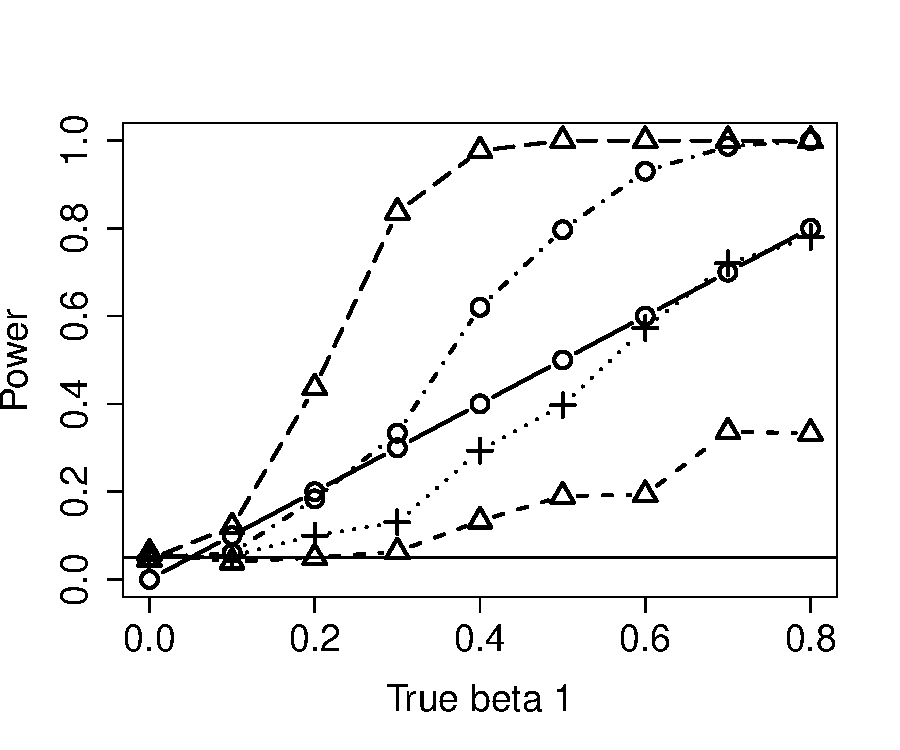
\includegraphics[width=\textwidth]{abs_perfor.pdf}
\centering
\caption{Power of the test statistic under the permutation test with significance level of 0.05.}
\end{figure}

\subsection{Resistance to outliers}

Multiple simulation studies were conducted to compute the power and type 1 errors of test statistics generated for a linear regression model with both squared loss and absolute loss under datasets with outliers. Table 2 and 3 show the value of type 1 error of test statistics generated under linear regression model with both squared loss and absolute loss with the significance level of $\alpha=0.05$. Figure 2 and 3 show the power curves of test statistics generated also under linear regression model with both squared loss and absolute loss with the significance level of $\alpha=0.05$. 

\begin{table}
\centering
\begin{tabular}{lllll}
\hline
Distribution & N=50 & N=100 & N=200 & N=500 \\
\hline
Laplace&  0.063& 0.088 &  0.04 & 0.162\\
Logistic &  0.068 & 0.064 &  0.051 & 0.047 \\
Cauchy &  0.186 & 0.159 &  0.133 & 0.141\\
$0.9 N(0, 3^2) + 0.1 N(0, 10^2)$ &  0.064 & 0.068  &  0.052 & 0.063\\
$0.8 N(0, 3^2) + 0.2 N(0, 20^2)$ &  0.083 & 0.078 &  0.065 & 0.045\\
$0.8 N(0, 3^2) + 0.2 N(0, 70^2)$ &  0.158 & 0.09  &  0.097 & 0.065\\
\hline
\end{tabular}
\caption{very basic table}
\label{tab:abc}
\end{table}

\begin{table}
\centering
\begin{tabular}{lllll}
\hline
Distribution & N=50 & N=100 & N=200 & N=500 \\
\hline
Laplace&  0.051& 0.046 &  0.053 & 0.049\\
Logistic &  0.046 & 0.054 &  0.046 & 0.048 \\
Cauchy &  0.046 & 0.051 &  0.06 & 0.035\\
$0.9 N(0, 3^2) + 0.1 N(0, 10^2)$ &  0.062 & 0.058  &  0.054 & 0.054\\
$0.8 N(0, 3^2) + 0.2 N(0, 20^2)$ &  0.056 & 0.063 &  0.056 & 0.063\\
$0.8 N(0, 3^2) + 0.2 N(0, 70^2)$ &  0.05 & 0.059  &  0.066 & 0.049\\
\hline
\end{tabular}
\caption{very basic table}
\label{tab:abc}
\end{table}

Though there are fluctuations of type 1 error value across different sample sizes and datasets generated from distributions, the only obvious outliers are type 1 errors of test statistic generated under linear regression model with squared loss and datasets generated by a Cauchy distribution. They reach the level of 0.15, which have largely exceeded the significance level of 0.05. Furthermore, the value of type 1 error tend to locate farther away from significance level as the sample size increases.


\begin{figure}[H]
     \begin{tabular}{cc}
     \centering
     \scalebox{0.45}{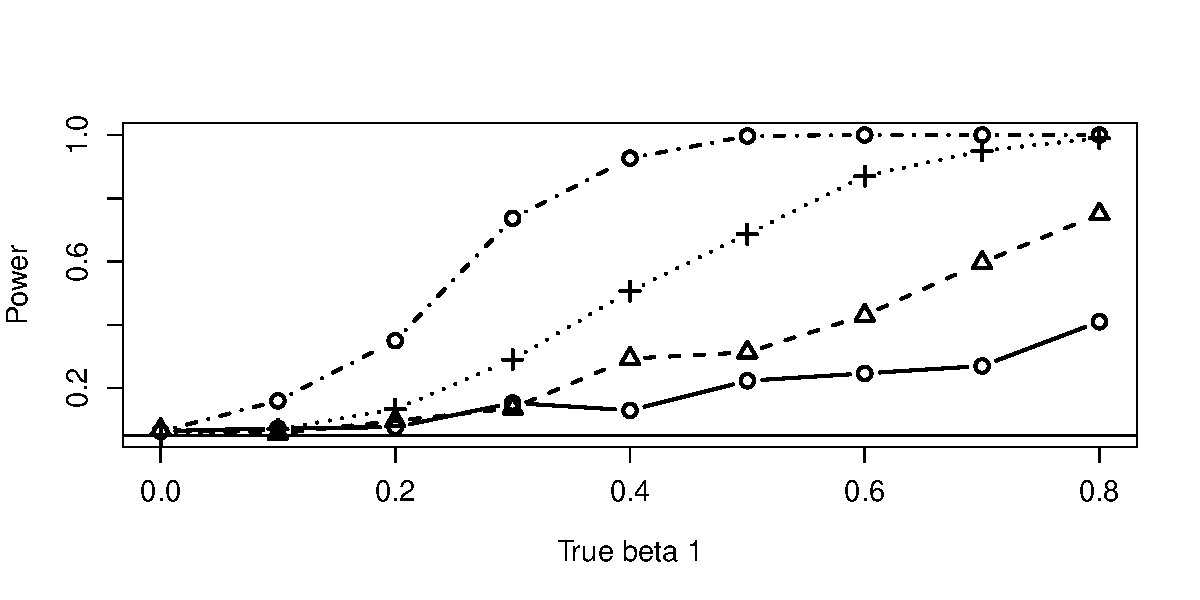
\includegraphics[width = 6in]{plt1_Li.pdf}} & \scalebox{0.45}{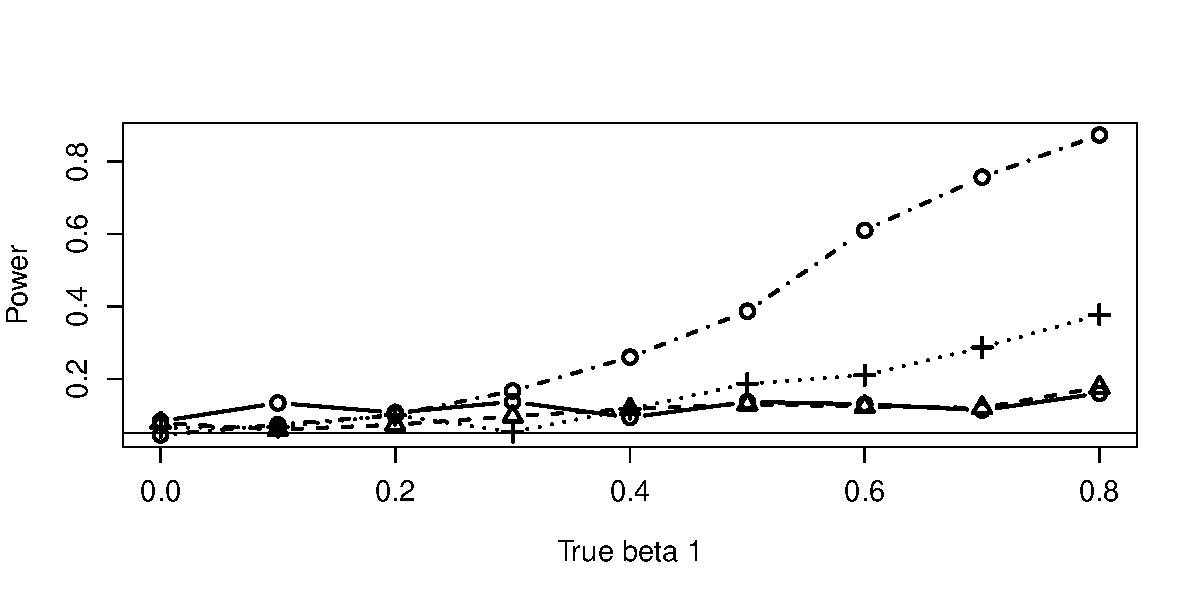
\includegraphics[width = 6in]{plt2_Li.pdf}} \\
     \scalebox{0.45}{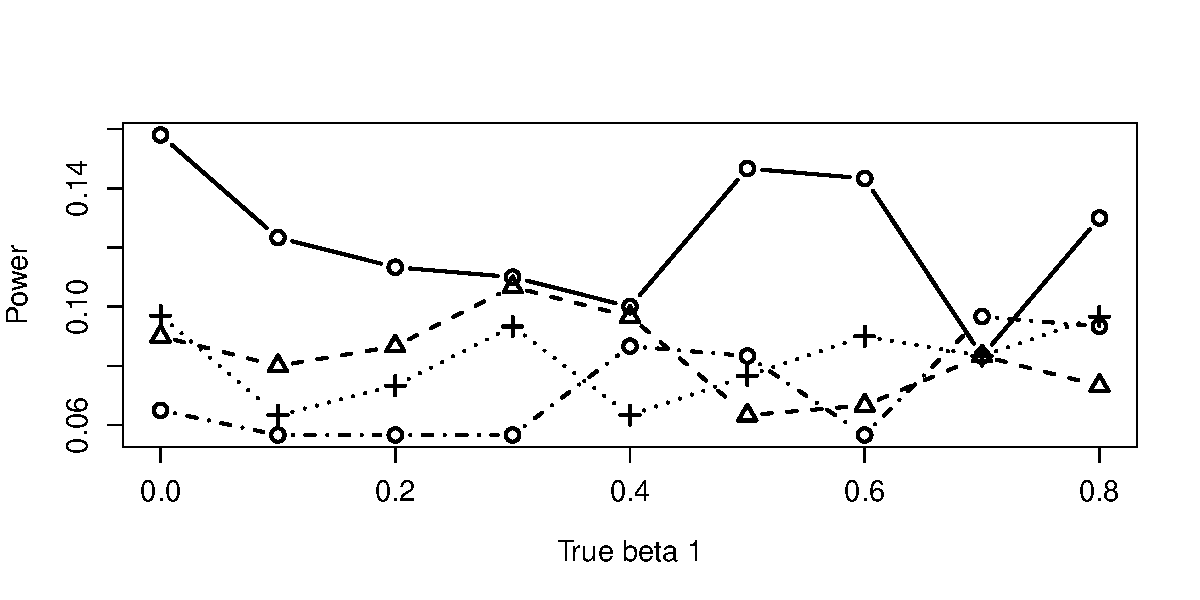
\includegraphics[width = 6in]{plt3_Li.pdf}} & \scalebox{0.45}{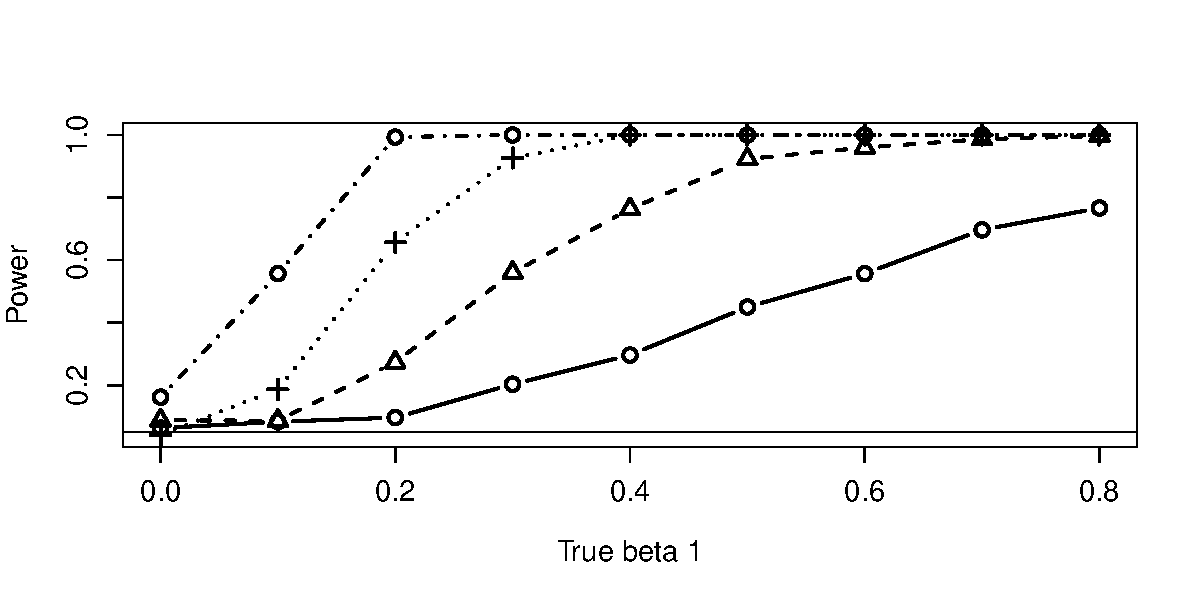
\includegraphics[width = 6in]{plt4_Li.pdf}} \\
     \scalebox{0.45}{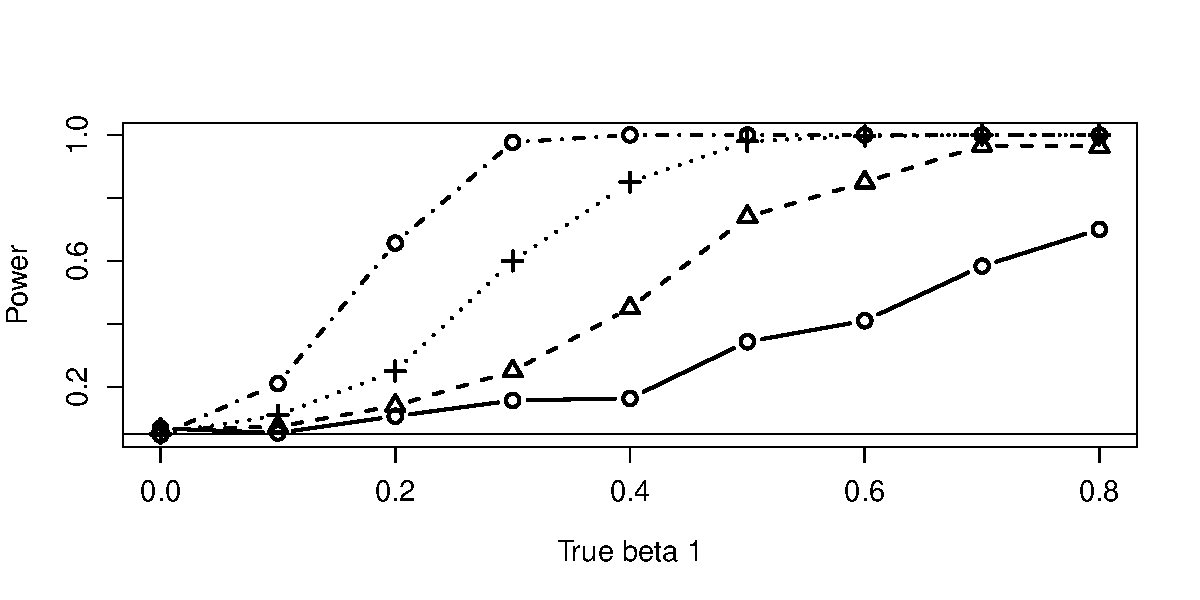
\includegraphics[width = 6in]{plt5_Li.pdf}} & 
\end{tabular}
\caption{Power of the proposed test under linear regression model with squared loss. Displayed are the power curves for Mixed distribution of 10\% data from normal distribution with s.d.=10 and 90\% data from normal distribution with s.d.=3 (top left),  Mixed distribution of 20\% data from normal distribution with s.d.=20 and 80\% data from normal distribution with s.d.=3 (top right), Mixed distribution of 20\% data from normal distribution with s.d.=70 and 80\% data from normal distribution with s.d.=3 (middle left),  Laplace distribution (middle right), and Logistic distribution (bottom left). The four curves in each figure represent four sample sizes: $n  =50$ (solid line with hollow circle), $100$ (dashed line with triangle), $200$ (dashed line with cross), and $500$ (dot-dashed line with hollow circles). }
\end{figure}


%%%%%%%%%%%%%%%%%
%% Original


\begin{figure}[H]
     \begin{tabular}{cc}
     \scalebox{0.45}{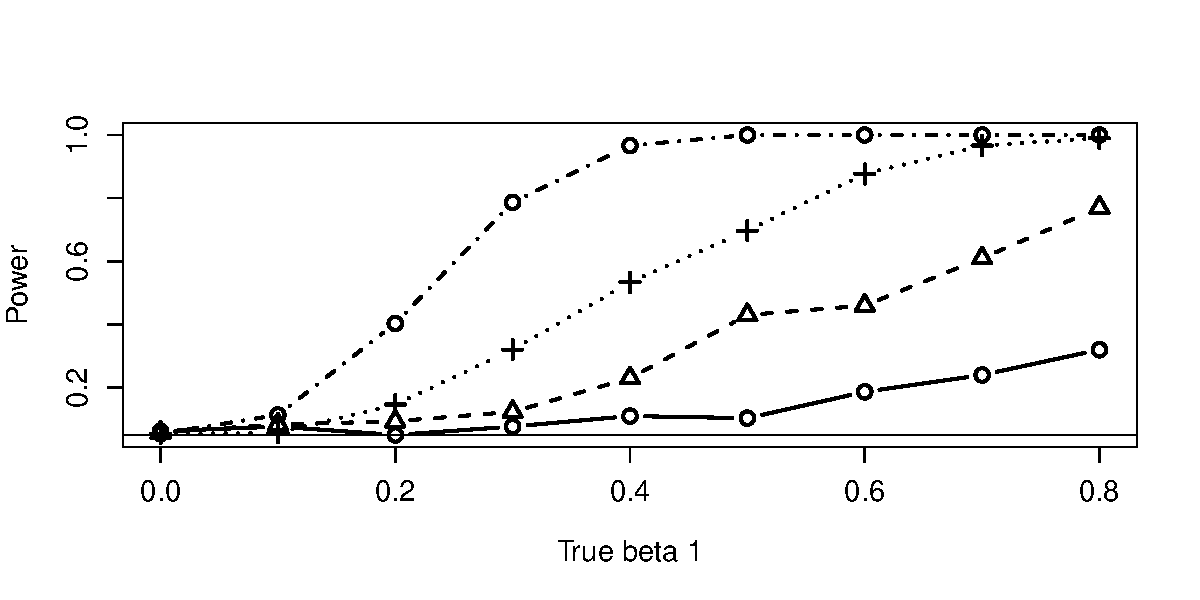
\includegraphics[width = 6in]{plt1_lo.pdf}} & \scalebox{0.45}{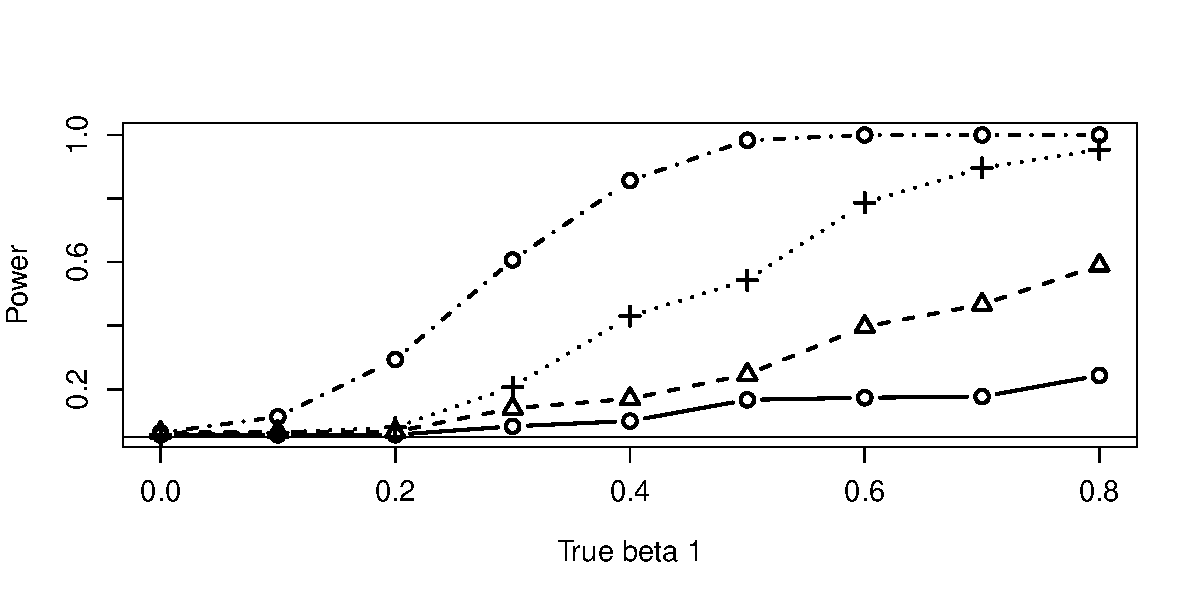
\includegraphics[width = 6in]{plt2_lo.pdf}} \\
     \scalebox{0.45}{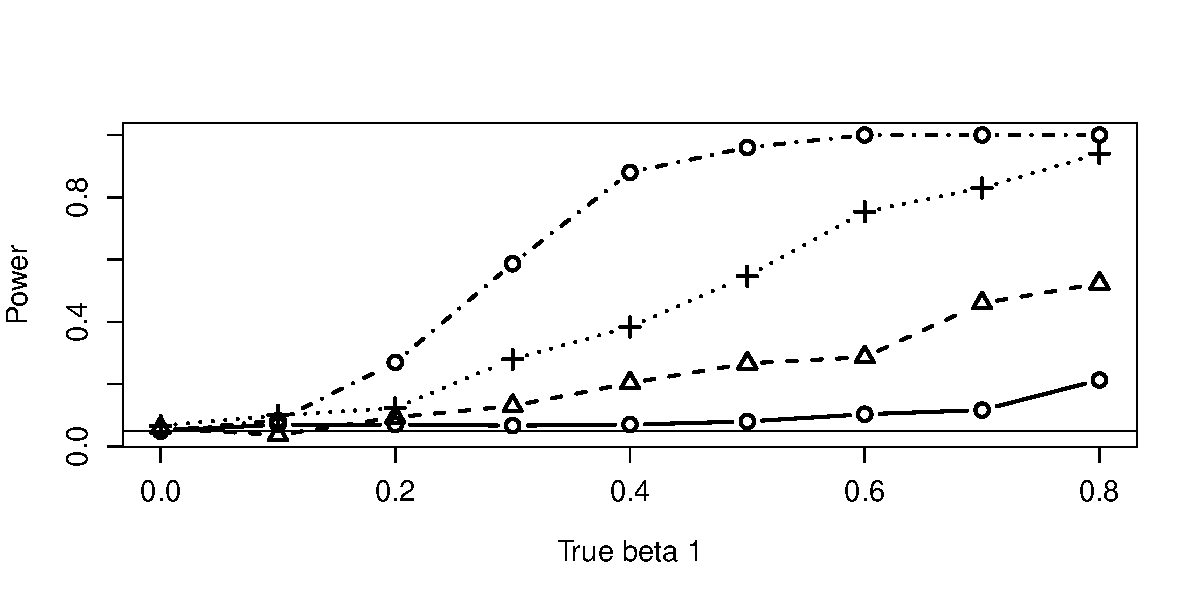
\includegraphics[width = 6in]{plt3_lo.pdf}} & \scalebox{0.45}{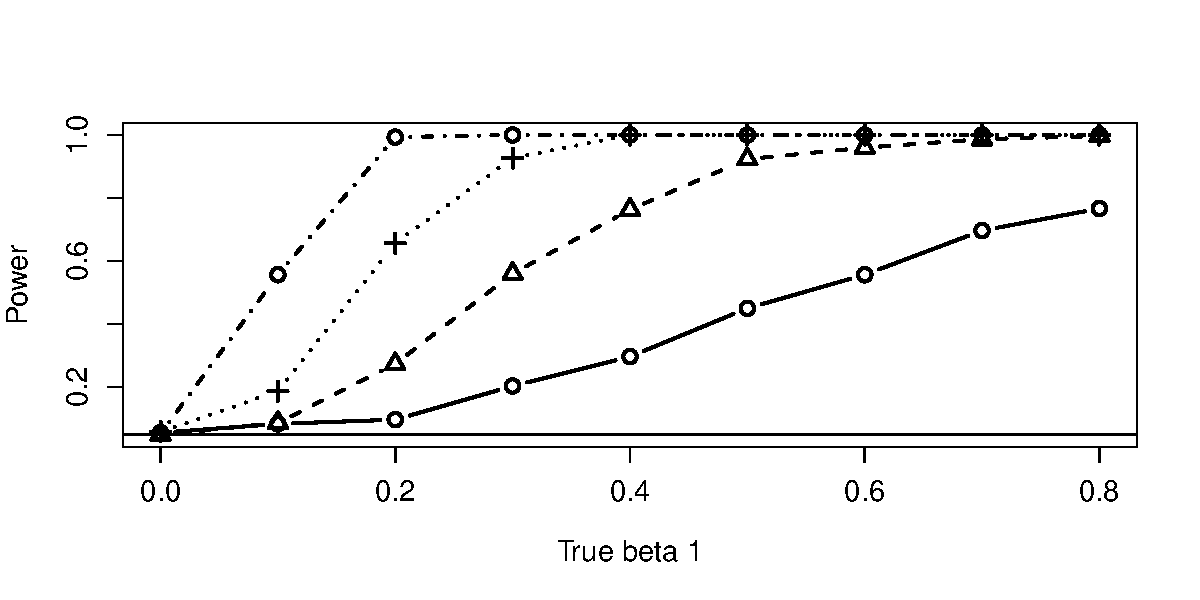
\includegraphics[width = 6in]{plt4_lo.pdf}} \\
     \scalebox{0.45}{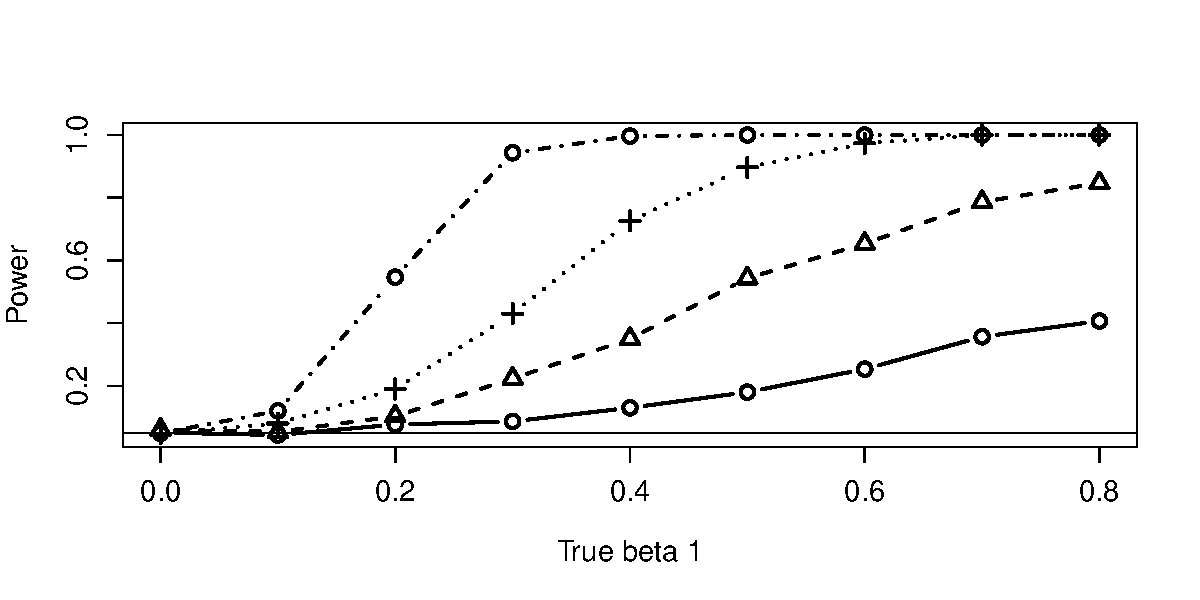
\includegraphics[width = 6in]{plt5_lo.pdf}} & 
     \scalebox{0.45}{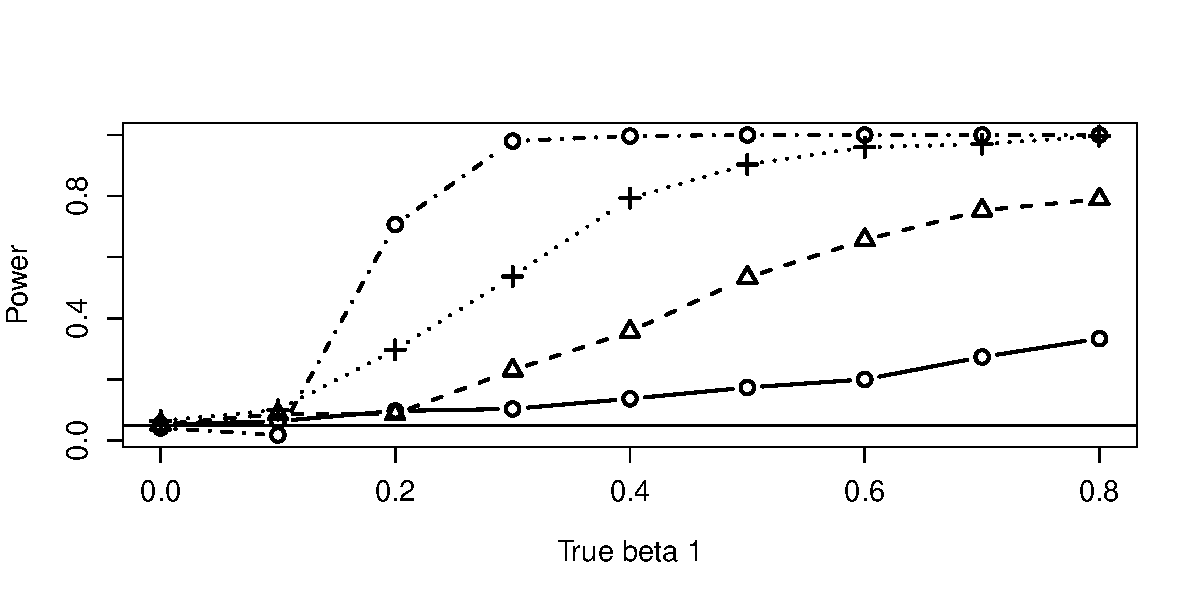
\includegraphics[width = 6in]{plt6_lo.pdf}}
\end{tabular}
\caption{Power of the proposed test under linear regression model with absolute loss. Displayed are the power curves for Mixed distribution of 10\% data from normal distribution with s.d.=10 and 90\% data from normal distribution with s.d.=3 (top left),  Mixed distribution of 20\% data from normal distribution with s.d.=20 and 80\% data from normal distribution with s.d.=3 (top right), Mixed distribution of 20\% data from normal distribution with s.d.=70 and 80\% data from normal distribution with s.d.=3 (middle left),  Laplace distribution (middle right), Logistic distribution (bottom left) and Cauchy distribution (bottom right). The four curves in each figure represent four sample sizes: $n  =50$ (solid line with hollow circle), $100$ (dashed line with triangle), $200$ (dashed line with cross), and $500$ (dot-dashed line with hollow circles). }
\end{figure}

Likewise, Power curves of most of these test statistics have the feature similar to power curves shown in figure 2d with an increasing trend when true value of $\beta_1$ grows from 0 to 0.8 and another increasing trend when sample size grows from 50 to 500. However, figure 3a, 3b and 3c exhibit the process of disappear power when an increasing number of extreme outliers are introduced to datasets. When the datasets were generated from 10\% of normal distribution with standard deviation of 10 and 90\% of normal distribution with standard deviation of 3, the power curves appear good. However, when the dataset was generated from 20\% of normal distribution with standard deviation of 70 and 80\% of normal distribution with standard deviation of 3, The power curves become horizontal lines. There were no powers under this kind of condition. Figure 2 and 3 also exhibit the trend that the power gradually disappears with more extreme outliers contained in the response. For example, with more percentage and more extreme of outliers geneated with mixed distribution, power curves become increasingly flat from figure 3a to 3c. It can also be observed from figure 3d to 3f, with the dataset generating function changes from Logistic distribution to Cauchy distribution.


\subsection{Real Data Analysis}

\section{Discussion}
In the paper, we developed a powerful hypothesis testing method for a Tukey 1-df interaction linear regression model. It can be widely used to evaluate contributions of target genes to a certain kind of continuous clinical measurement with gene-gene and gene-environment interactions. By considering the hypothesis testing method proposed for logistic regression model with binary clinical measurement as responses, we are motivated to introduce the hypothesis testing protocol to linear regression model. We derived the test statistic for the hypothesis testing and finished the testing with permutation test that permute residuals under reduced model. To avoid some of the potential risk when dataset contains extreme outliers, we introduced absolute loss function to derive calculate the score function and information matrix during the process of test statistic derivation. We conducted extensive simulation studies to test the performance of the test statistic and the performance of testing using absolute loss to resist outliers. The test statistic performs very well under the permutation test with pre-set parameters with reasonable type I error rate and power curves. Both tests using squared loss and absolute loss performed well when facing moderate outliers. However, when facing extreme outliers in the response, test using squared loss encountered serious problems either with collapsed power or high type I error while test using absolute loss retains its power.

\section{References}
Freedman, D., \& Lane, D. (1983). A nonstochastic interpretation of reported significance levels. \textit{Journal of Business \& Economic Statistics, 1}(4), 292-298.

Gibbs, R. A., Belmont, J. W., Hardenbol, P., Willis, T. D., Yu, F. L., Yang, H. M., ... \& Duster, T. (2003). The international HapMap project..

Hindorff, L. A., Sethupathy, P., Junkins, H. A., Ramos, E. M., Mehta, J. P., Collins, F. S., \& Manolio, T. A. (2009). Potential etiologic and functional implications of genome-wide association loci for human diseases and traits. \textit{Proceedings of the National Academy of Sciences, 106}(23), 9362-9367.

Jablonski, K. A., McAteer, J. B., de Bakker, P. I., Franks, P. W., Pollin, T. I., Hanson, R. L., ... \& Diabetes Prevention Program Research Group. (2010). Common variants in 40 genes assessed for diabetes incidence and response to metformin and lifestyle intervention in the diabetes prevention program. \textit{Diabetes, 59}(10), 2672-2681.

Jia, Y., McAdams, S. A., Bryan, G. T., Hershey, H. P., \& Valent, B. (2000). Direct interaction of resistance gene and avirulence gene products confers rice blast resistance. \textit{The EMBO journal, 19}(15), 4004–4014.

Michailidou, K., Hall, P., Gonzalez-Neira, A., Ghoussaini, M., Dennis, J., Milne, R. L., ... \& Devilee, P. (2013). Large-scale genotyping identifies 41 new loci associated with breast cancer risk. \textit{Nature genetics, 45}(4), 353-361.

Mukherjee, B., Ahn, J., Gruber, S. B., \& Chatterjee, N. (2012). Testing gene-environment interaction in large-scale case-control association studies: possible choices and comparisons. \textit{American journal of epidemiology, 175}(3), 177-190.

Titeca, K., Lemmens, I., Tavernier, J., \& Eyckerman, S. (2019). Discovering cellular protein‐protein interactions: Technological strategies and opportunities. \textit{Mass spectrometry reviews, 38}(1), 79-111.

Tukey, J. W. (1949). One degree of freedom for non-additivity. \textit{Biometrics, 5}(3), 232-242.

Wang, Y., Li, D., \& Wei, P. (2015). Powerful Tukey's One Degree-of-Freedom Test for Detecting Gene-Gene and Gene-Environment Interactions. \textit{Cancer informatics, 14}, CIN-S17305.



\end{document}
